\section{Method}
\label{sec:method}
In this section, we will first define our task and weighted decoding method for controllable generation as background. Then we will introduce the proposed \textbf{DASC} framework. 
\subsection{Task Definition}

Given a dialogue \textbf{context} $C$ and \textbf{attributes} $A = (a_1, a_2, ..., a_K)$, \textit{Controllable Dialogue generation} aims to generate a \textbf{response} $R = (r_1, r_2, ..., r_N)$ that both cohere with the context and convey the attributes. 
% \KZ{You seem to confuse attributes with aspects. Actually your aspects are the attributes, and your attributes are the attribute values. E.g., Gender is an attribute (or attribute type), male or female is an attribute value.  No need to mention aspects.}
% \ZL{Just two potential ways to present the terms. I choose aspect/attribute instead of attribute/attribute values following some previous works, and sticks to it throughout the paper. 0/1/$\phi$ is the attribute value here.}
\footnote{In our work, we make a pre-assumption that attributes 
are provided by a dialogue policy, and do not include end-to-end scenarios.}
There can be multiple \textbf{aspects} grouping the attributes, where in this work we will focus on \textit{Gender Style, Emotion, and Dialogue Act}. An aspect covers multiple related attributes, such as \textit{happiness, sadness} for the Emotion aspect. Each attribute can take three values: 1 means to use the attribute, 0 means not to use and $\phi$ means the attribute has no effect on the response.

% \KZ{What do u mean by this: end-to-end scenarios}
% \ZL{Generate the response directly without using explicit attributes in the system.}

\subsection{Weighted Decoding for Controllable Generation}
\label{sec:weighted_decoding}

Generally, dialogue generation can be formulated with the standard conditional language modeling objective:

\begin{equation}
    L_{CLM} = -\sum_{n=1}^N log P(r_n|r_{1:n-1}, C)
\end{equation}

We can use a transformer-based encoder-decoder architecture like BART \cite{lewis2020bart} to model this, where the encoder encodes the context into hidden states as condition for the decoder to generate the response. We will omit $C$ below for brevity.

In controllable dialogue generation, we additionally introduce attributes in the generation condition. Suppose we are generating with a single attribute $a$, then the objective is to model $P(r_n|r_{1:n-1}, a)$. Using Bayes' rule, this can be converted to:
% \KZ{It's not good to use small font for equations. Note that the equation
% numbers have also been shrunk and inconsistent across the paper (some big,
% some small).}
\begin{equation}
    \small
    P(r_n|r_{1:n-1}, a) \propto P(r_n|r_{1:n-1}) P(a|r_{1:n-1}, r_n)^{\alpha}
    \label{eqn:single_wd}
\end{equation}
where $\alpha$ is a hyperparameter that can adjust the \textit{control strength}. This means that we can decompose the generation probability into the standard CLM probability weighted by the prediction of another token-wise attribute classifier during decoding. Methods established on such decomposition are thus called \textbf{Weighted Decoding} models.

Director \citep{arora2022director}, a representative weighted decoding method, implements the attribute classifier as a linear layer on top of the decoder hidden states. It performs the binary classification whether the full generation will reflect the desired attribute  (e.g. happy or not) at each step. For tokens in the sentence from training set, they can be trained with the attribute of the whole sentence using Binary Cross Entropy (BCE) loss. We denote this token-level loss as $L_{clf-t}$. 

\begin{equation}
    \begin{aligned}
        L_{clf-t} &= BCE(P(a | r_{1:n-1}, r_n)) \\
                  &= BCE(\sigma([W_a h_n]_{r_n}))
    \end{aligned}
    \label{eqn:clf_t}
\end{equation}
where $h_n \in \mathbb{R}^{d}$ is the hidden state for the $n$-th token, $W_a \in \mathbb{R}^{|V| \times d}$ is the learnable weight matrix for attribute prediction given the generation of each token in the vocabulary, and $[*]_{r_n}$ denotes the index selection with the next token $r_n$. Note that it only gathers the attribute logits with $r_n$ according to the ground truth response. However, for the other $|V|-1$ tokens in the vocabulary $V$, they have no label and cannot get trained. Therefore, it uses an extra regularizer to train the prediction on these tokens' to be close to 0.5 with MSE loss.  

When dealing with multi-attribute control, we can extend \eqnref{eqn:single_wd} by introducing the product of multiple attribute classifiers, assuming the conditional independence of attributes:

\begin{equation}
    \small
    P(r_n|r_{1:n-1}, a) \propto P(r_n|r_{1:n-1}) \prod_{\substack{k=1\\a_k\ne \phi}}^{K} P(a_k|r_{1:n})^{\alpha}
    \label{eqn:multi_wd}
\end{equation}

The product of probabilities is usually implemented with the summation of logits: 

\begin{equation}
    \small
    \delta(r_n|r_{1:n-1}, a) = \delta(r_n|r_{1:n-1}) + \alpha \sum_{\substack{k=1\\a_k\ne \phi}}^{K} \delta(a_k|r_{1:n})
    \label{eqn:multi_wd_logits}
\end{equation}

We may implement such an extension with multiple forward passes through an attribute-conditioned language model \citep{lin2021plug} or one pass of multiple models \citep{liu2021dexperts}. Here we introduce a relatively simple and efficient implementation in a similar form as Director, where we just add $K$ linear classifier heads to make the prediction of multiple attributes. We will refer to this simple extension as M-Director, or just Director for simplicity. Note that such a model will still introduce $[d, |V|, K]$ extra parameters. Given that $|V|$ is usually as large as tens of thousands, this model will have numerous parameters, which makes the model inefficient to train or infer, and also prone to overfitting.

\subsection{Dialogue Attribute Space Controller}
\label{sec:dasc_method}
We hypothesize that such typical methods of weighted decoding may not be the most effective approach to learn the token-level attribute semantics, especially in multi-attribute cases. The learning objective is imposed on discrete token-level, and only the single token in the target sentence gets a distinctive training signal, and other tokens are regularized equally. This is not usually reasonable, as some tokens similar to the target token should also have high probabilities given the attribute while other tokens different from it are less likely to be generated. For example, in a \textit{happy} response ``Nice to meet you'', ``glad'' will also be a reasonable alternative for the first word with the same emotion, while ``sad'' is not acceptable, but their attribute label in training will both be 0.5.

We can implement this intuition in a high-dimensional space. On one hand, each token has an embedding that encodes its attribute semantics (\textit{Attribute Token Embedding}, $ATEMB$). On the other hand, the hidden states from the LM ($h_n$) are also projected to the same space with attribute-specific linear layers ($W^k \in \mathbb{R}^{p \times d}$) to get \textit{Attribute Context Embedding}. Formally, $\hat h^k_n = \hat W^k h_n$. Then the representations in the space will convey the semantics, and we call it \textit{Attribute Semantic Space}. 

To leverage this latent space for weighted decoding, for each $\hat h^k_n$, we find its attribute-related tokens according to embedding similarity in the space, and assign them higher weights during decoding. Specifically, it is accomplished with a dot-product based token-level attribute classifier.


\begin{equation}
    \small
    \delta(a_k|r_{1:n}) = \hat h^k_n \cdot ATEMB(r_n)
    \label{eqn:matching_for_logits}
\end{equation}

In this case, when a token is trained with high probability for 
certain attribute, its neighbors in the attribute space will also 
have higher probabilities. This alleviates the limitation of previous 
weighted decoding methods, and eliminates the need for regularizers on 
other tokens. Further, when applying this to multi-attribute weighted decoding, 
we get: 

\begin{equation}
    \small
    \begin{aligned}
        \delta(r_n|r_{1:n-1}, a) &= \delta(r_n|r_{1:n-1}) \\
                                 &+ \alpha K (\frac{1}{K} \sum_{\substack{k=1\\a_k\ne \phi}}^{K} \hat h^k_n) \cdot ATEMB(r_n)
    \end{aligned}
    \label{eqn:dasc_logits}
\end{equation}
where the parenthesis part in the second term can be interpreted as the average/equal-weight interpolation of multiple attribute context embeddings. 
\footnote{It is possible to assign different weights for each embedding in interpolation, and we leave it for future works.}
This formulation suggests that if the attribute space is properly learned and represented, the embedding interpolation will precisely reflect the semantics of the desired attributes, and then DASC can realize reasonable attribute combinations. 

\begin{figure}[t]
    \centering
    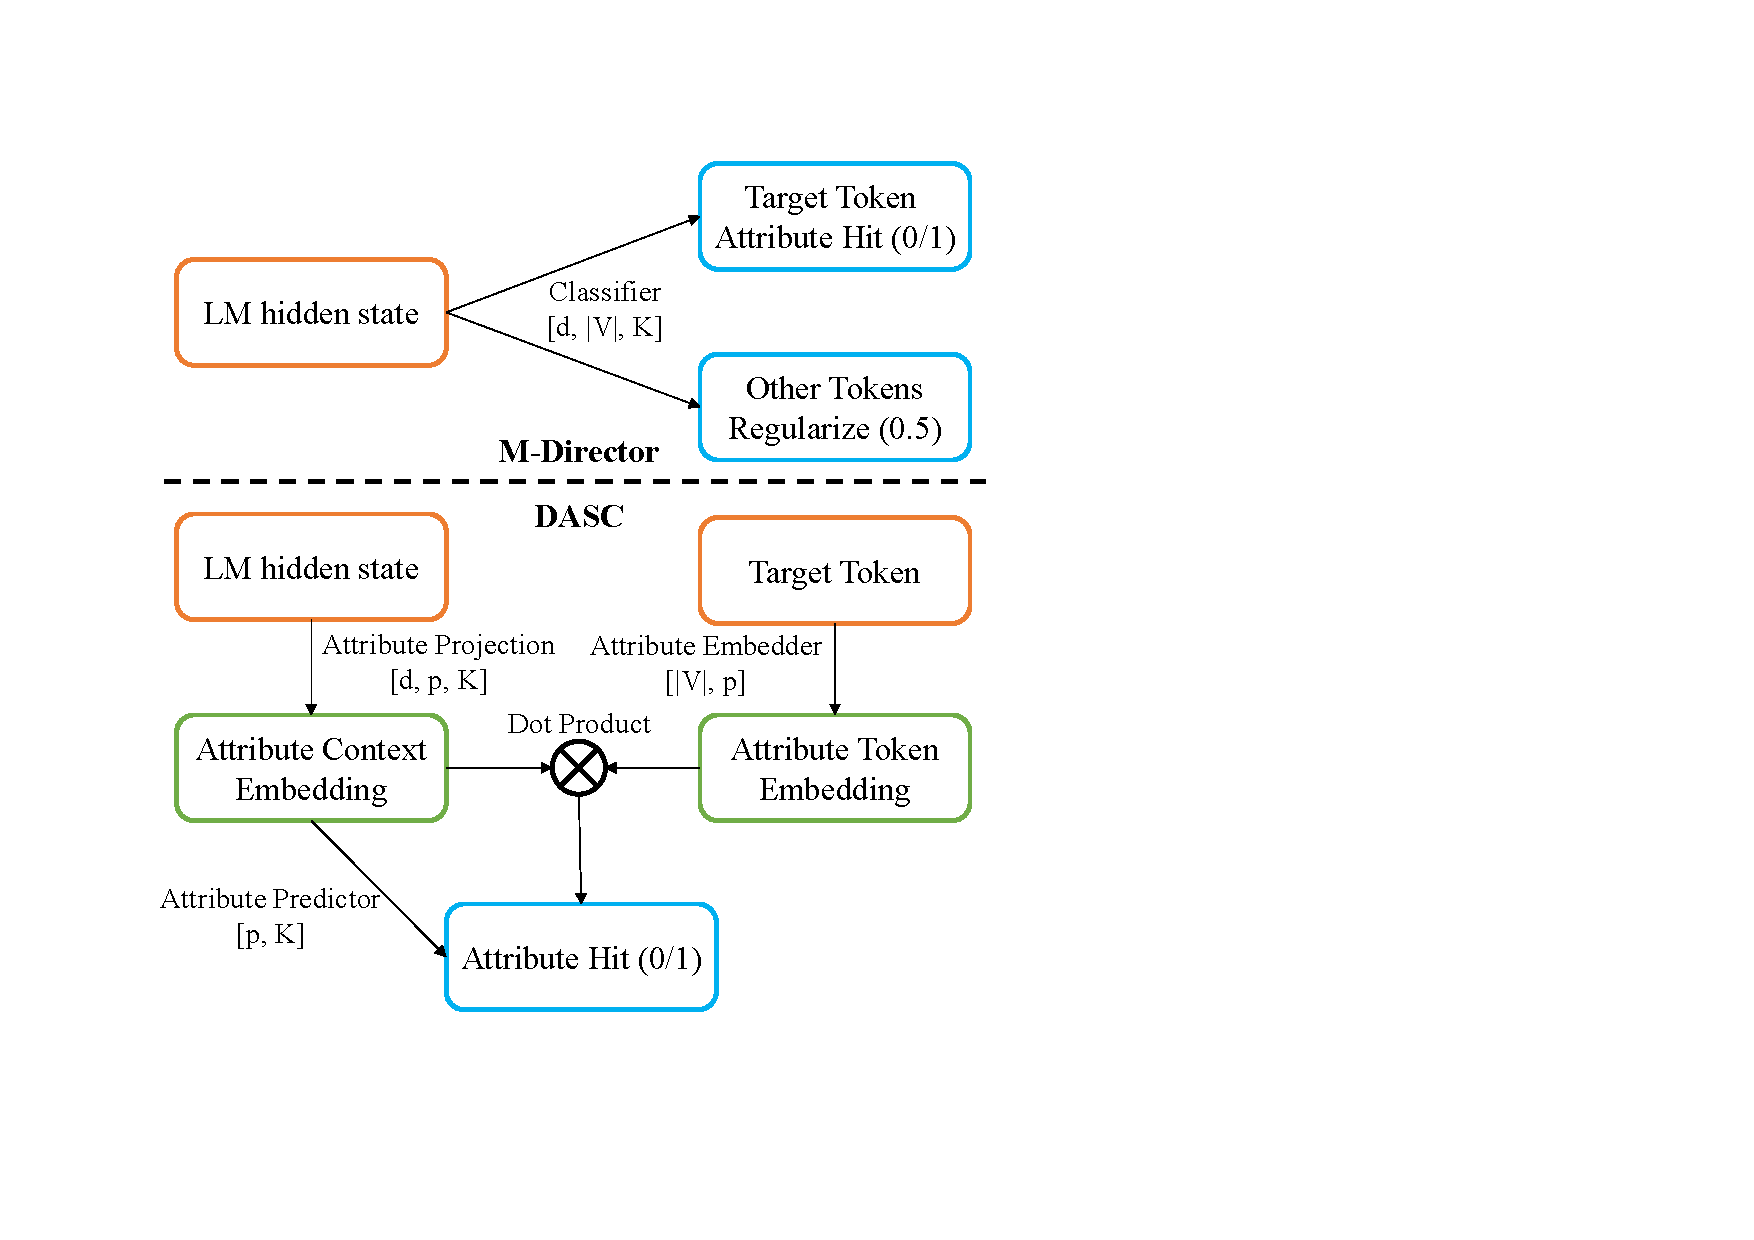
\includegraphics[width=1.0\columnwidth]{figures/dasc_illustration.pdf}
    \caption{Framework comparison between M-Director and DASC. M-Director uses a classifier head to conduct binary attribute hit classification for each token in the target sentence, and impose regularization for other tokens. 
DASC projects both LM hidden state and the target token to the attribute space, and uses their dot product for the classification of attribute hit. 
For each parameterized model component, we show its shape in square brackets.}
    \label{fig:dasc_illustration}
\end{figure}

To assist the learning of attribute embeddings, we introduce another linear layer on top of the attribute context embedding at each step to directly predict the attributes of the complete response. This can help better align the attribute context embeddings to the corresponding region for its attributes. We denote the new the sentence-level classification loss as $L_{clf-s}$. For clarity, we give its formulation in the single-attribute case, which can be simply extended to multi-attribute scenarios with the summation over all non-empty attributes.

\begin{equation}
    \begin{aligned}
        L_{clf-s} &= BCE(P(a | r_{1:n-1})) \\
                  &= BCE(\sigma(v_a \cdot \hat h_n))
    \end{aligned}
\end{equation}
where $v_a \in \mathbb{R}^{p}$ is the learnable weight for attribute prediction. Compared with $L_{clf-t}$ (\eqnref{eqn:clf_t}), it is a sentence-level classification task independent of $r_n$, which can also be interpreted as predicting the prior probability of the attribute before deciding the next token to generate, and thus the parameters do not scale with $|V|$. Then the final loss is: 

\begin{equation}
    L_{train} = L_{LM} + \beta (L_{clf-s} + L_{clf-t})
\end{equation}
where $\beta$ is a hyperparameter that controls the weight of attribute-related losses.

We name the proposed framework as Dialogue Attribute Space Controller (\textbf{DASC}). The illustration of DASC and its comparison with M-Director is shown in Figure \ref{fig:dasc_illustration}. DASC introduce fewer parameters than M-Director ($[d, |V|, K]$). Since we usually set $p$ close to $d$ ($d << |V|$), the parameters of attributes projections will be much smaller. And when we deal with $K > 1$, the shared token embeddings across attributes will also save parameters, while the parameters of attribute predictor are almost negligible. As we will validate in Sec. \ref{sec:parameter_analysis}, the suitable amount of parameters also helps DASC achieve a better balance between controllability and generation quality. 
% \MY{This balance between controllability and quality can be made more obvious in your intro part}

% \KZ{It would be better to use different shapes to represent different type of
% nodes. If you put functions, processes on top of an arrow, the problem is
% your function can't take more than 1 argument. The two arrows at the bottom are a bit misleading.}
